\documentclass[varwidth=true, border=2pt]{standalone}

\usepackage{pgfplots}
\usepackage{tikz}
\usepackage{amsmath}
\usepackage{amssymb}

\usetikzlibrary{calc,patterns,angles,quotes}

\newcommand{\R}{\mathbb{R}}

\begin{document}
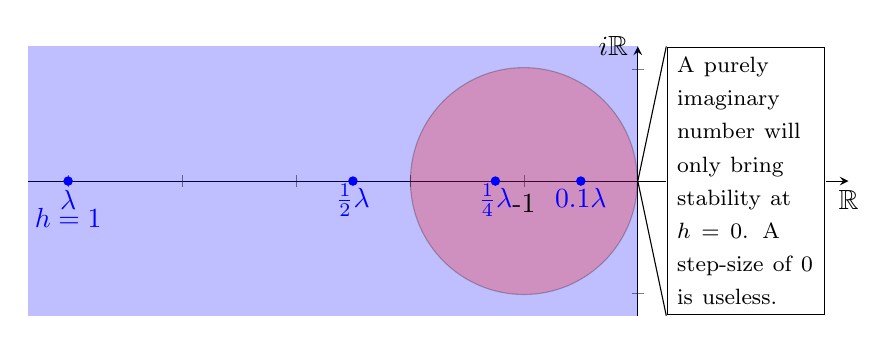
\begin{tikzpicture}
    \begin{axis}[
        legend pos=south east,
        axis x line=middle,
        axis y line=middle,
	every axis x label/.style={at={(current axis.right of origin)},anchor=north},
	every axis y label/.style={at={(current axis.above origin)},anchor=east},
	xticklabels=\empty,
	yticklabels=\empty
        grid = none ,
        width=12cm,
        height=5cm,
        grid style={dashed, gray!1},
        xmin=-4.75,
        xmax=1.25,
        ymin=-1,
        ymax=1,
        xlabel=$\R$,
        ylabel=$i \R$,
        enlargelimits=true,
        tension=0.08]

	
	\draw [fill=blue, opacity=0.25] (axis cs: -6,2) rectangle (axis cs: 0, -2);
	\filldraw [fill= red, opacity = 0.25] (axis cs: -1,0) circle (41pt);
	\node(X1) at (axis cs: -1, -0.2){-1};
	\node (L1)[blue] at (axis cs: -0.5, -0.15) {$0.1 \lambda$};
	\node (L2)[blue] at (axis cs: -1.25, -0.17) {$\frac{1}{4} \lambda$};
	\node (L3)[blue] at (axis cs: -2.5, -0.17) {$\frac{1}{2} \lambda$};
	\node (L4)[blue] at (axis cs: -5, -0.17) {$\lambda$};
	\node (L5)[blue] at (axis cs: -5, -0.33) {$h = 1$};
	\node (O) at (axis cs: 0,0){};
	\node (O1) at (axis cs: 0.25, 1.2){};
	\node (O2) at (axis cs: 0.25, -1.2){};
	\node (O3) at (axis cs: 1.65, -1.5){};
	\filldraw [white, fill = white] (O1) rectangle (O3);
	\draw (O1.center) to (O.center);
	\draw (O2.center) to (O.center);
	\node(X2)[draw,text width = 1.75cm] at (axis cs: 0.95, 0){\footnotesize{A purely imaginary number will only bring stability at $h = 0$.
		A step-size of 0 is useless.}};	
	
	\addplot[blue, only marks, mark=*, mark size=1.5pt] coordinates{
	(-0.5,0)(-1.25,0)(-2.5,0)(-5,0)};
	

    \end{axis}
\end{tikzpicture}
\end{document}